\documentclass[12pt,a4paper]{article}
\usepackage[utf8]{inputenc}
\usepackage[T1]{fontenc}
\usepackage{amsmath, amssymb}
\usepackage{graphicx}
\usepackage{booktabs}
\usepackage{array}
\usepackage{tabularx}
\usepackage{adjustbox}
\usepackage{xcolor}
\usepackage{float}
\usepackage{tikz}
\usetikzlibrary{arrows.meta, positioning, shapes.geometric, fit, backgrounds}
\usepackage{geometry}
\geometry{margin=1in}
\usepackage{hyperref} % load last-ish
\hypersetup{colorlinks=true, linkcolor=blue!50!black, urlcolor=blue!50!black, citecolor=blue!50!black}

% ---------------------------------------------------------------------------
% Measured results. Every \R... macro below is OVERWRITTEN by
% results/results_macros.tex, which the notebook (Step 10b) generates.
% If you see red ?? in the PDF, the notebook has not been run yet.
% ---------------------------------------------------------------------------
\newcommand{\defres}[1]{\expandafter\newcommand\csname R#1\endcsname{\textcolor{red}{\textbf{??}}}}
\defres{DenseModel}\defres{DenseBackend}\defres{FinalMethod}\defres{DenseFeature}
\defres{TauDense}\defres{TauCov}\defres{TauOOD}\defres{TuneObjective}\defres{TuneGrid}\defres{TunePlateau}
\defres{NPassages}\defres{NDocs}\defres{NRecords}\defres{NDev}\defres{NDevOfficial}\defres{NDevAux}
\defres{NTest}\defres{NTestGold}\defres{NBrief}\defres{DatasetHash}
\defres{TestRecall}\defres{TestRecallCI}\defres{TestMRR}\defres{TestMRRCI}\defres{TestHitOne}
\defres{BaseRecall}\defres{BaseMRR}
\defres{DecAcc}\defres{DecAccCI}\defres{AnsPrec}\defres{AnsRec}\defres{AnsFOne}\defres{FalseAns}
\defres{ClarifyAcc}\defres{NAnswerable}\defres{NUnanswerable}
\defres{CiteSupport}\defres{CiteSupportCI}\defres{VerifierPass}\defres{CitedGold}\defres{NAnswered}\defres{AnswerFOneOverlap}
\defres{LatPfifty}\defres{LatPninetyfive}\defres{LatMean}
\defres{CrossTopOne}\defres{CrossAllHit}\defres{CrossJaccard}\defres{CrossSV}\defres{EtoECrossDec}\defres{EtoECrossCite}
\defres{LeakForms}\defres{LeakRecallWithout}\defres{LeakMRRWithout}\defres{LeakCues}\defres{CueAccWithout}\defres{CueFalseWithout}
\defres{BriefAcc}\defres{DevAcc}\defres{NErrors}\defres{BlindStatus}\defres{StyleAcc}
\InputIfFileExists{results/results_macros.tex}{}{}

% table / figure helpers that degrade gracefully before the notebook is run
\newcommand{\resmissing}[1]{\fbox{\parbox{0.8\textwidth}{\centering\small
  Run the notebook (Step 10b) to generate \texttt{\detokenize{#1}}.}}}
\newcommand{\restable}[1]{\IfFileExists{results/#1.tex}{\input{results/#1.tex}}{\resmissing{results/#1.tex}}}
\newcommand{\restablefit}[1]{\IfFileExists{results/#1.tex}{\begin{adjustbox}{max width=\linewidth}\input{results/#1.tex}\end{adjustbox}}{\resmissing{results/#1.tex}}}
\newcommand{\resfig}[2]{\IfFileExists{results/figs/#1}{\includegraphics[width=#2]{results/figs/#1}}{\resmissing{results/figs/#1}}}

\title{Multilingual E-Sahulat AI:\\[2pt] \large Evidence-Grounded Multilingual Retrieval and Answering\\ for Pakistani Passport Services}
\author{Team Name --- Member 1, Member 2, Member 3\\ \small TexTrek NLP Hackathon}
\date{\today}

\begin{document}

\maketitle

\begin{abstract}
\noindent
We present \textit{Multilingual E-Sahulat AI}, an evidence-grounded assistant that answers questions about Pakistani
passport services asked in Urdu script, Roman Urdu, English, or a mix of these. The system normalizes queries across scripts,
bridges them to official English passages with a cross-script concept lexicon, retrieves evidence with keyword, character
n-gram, multilingual dense and hybrid retrievers, and answers \emph{extractively}, quoting the official passage with its
source URL. When evidence is missing, the question is ambiguous or the request is unsafe, it abstains or asks for
clarification. On the organisers' official test split (\RNTest{} queries) the production retriever (\RFinalMethod) reaches
Recall@5 = \RTestRecall{} \RTestRecallCI{} and MRR@5 = \RTestMRR{}, against \RBaseRecall{} / \RBaseMRR{} for a raw BM25 baseline.
End-to-end decision accuracy is \RDecAcc{} with a false-answer rate of \RFalseAns{} on unanswerable queries and a citation
support rate of \RCiteSupport{}. Because the test queries were visible during development, we also report conservative,
leakage-ablated figures (\S\ref{sec:leakage}). No external APIs or generative models are used.
\end{abstract}

\tableofcontents
\newpage

% =====================================================================================
\section{Introduction}
Pakistan's public-service information sits on official websites, FAQs and procedural pages that are written mostly in
English or formal Urdu. Citizens, however, ask in Urdu script, in Roman Urdu with highly variable spelling
(\textit{pasport renu karwana hy}), in English, or in code-mixed sentences. Keyword search breaks when the query's script or
spelling differs from the source, and generative chatbots can produce fluent but unsupported answers about legal
requirements.

This project builds a \textbf{retrieval-first, extractive} assistant for one well-defined domain, \textbf{DGI\&P ordinary
passport services}, with three goals taken from the challenge brief:
\begin{enumerate}
  \item retrieve the correct official evidence regardless of script, spelling or paraphrase;
  \item answer \emph{only} what that evidence supports, with a traceable citation;
  \item abstain or ask for clarification when the evidence does not support an answer, and measure all of this
        quantitatively on a documented test set.
\end{enumerate}

% =====================================================================================
\section{System Overview}
The pipeline consists of the following steps (Figure~\ref{fig:flow}):

\begin{enumerate}
    \item \textbf{Question input and language selection:} the user submits a question and picks a response language
          (English, Urdu, Roman Urdu, or automatic detection).
    \item \textbf{Normalization:} Unicode NFKC, Arabic$\to$Urdu letter unification, diacritic and digit normalization,
          Roman Urdu elongation and spelling-variant repair.
    \item \textbf{Concept analysis:} a cross-script lexicon maps surface forms to concepts (e.g.\ \textit{tajdeed / renu /
          renew} $\to$ \texttt{RENEW}) and adds English expansion terms from the corpus vocabulary.
    \item \textbf{Retrieval:} BM25 over bilingual passages plus multilingual dense retrieval (\RDenseModel), fused by
          Reciprocal Rank Fusion. The production configuration is selected on the development split.
    \item \textbf{Decision cascade:} rule gates (injection, unsafe, personal or guarantee requests, out-of-scope, ambiguity)
          followed by evidence thresholds tuned on development data.
    \item \textbf{Grounded answer:} the official passage is quoted verbatim with its passage ID, title and URL. A citation
          verifier checks the quote, the URL and every number.
    \item \textbf{Output:} a structured response (decision, reason, message, evidence, notes, and a trace for inspection).
\end{enumerate}

Table~\ref{tab:tech} summarizes the technologies used.

\begin{table}[H]
\centering
\begin{tabular}{@{}>{\raggedright}p{3.4cm}>{\raggedright}p{5.6cm}>{\raggedright\arraybackslash}p{5.0cm}@{}}
\toprule
Component & Technology / Model & Purpose \\
\midrule
Normalization & Python \texttt{unicodedata}, regex rules & Script and spelling robustness \\
Spelling repair & \texttt{difflib} similarity ($\geq 0.84$) & Roman Urdu variant recovery \\
Concept lexicon & 50+ cross-script concepts & Urdu/Roman$\to$English bridging \\
Sparse retrieval & BM25Okapi (own implementation) & Keyword matching \\
Char retrieval & scikit-learn char 3--5-gram TF-IDF & Spelling-robust baseline \\
Dense retrieval & \RDenseModel{} (local, MIT) & Multilingual semantic matching \\
Fusion & Reciprocal Rank Fusion ($k=60$) & Hybrid ranking \\
Decision layer & Rule gates + dev-tuned thresholds & Abstention / clarification \\
Answering & Extractive quoting + verifier & No unsupported claims \\
Evaluation & NumPy, Pandas, bootstrap CIs & Metrics and error analysis \\
Visualization & Matplotlib & Report plots \\
Deployment & Jupyter / Colab (CPU or GPU) & Reproducible notebook \\
\bottomrule
\end{tabular}
\caption{Technologies and techniques used. No external API is called; all models are loaded locally.}
\label{tab:tech}
\end{table}

\begin{figure}[H]
\centering
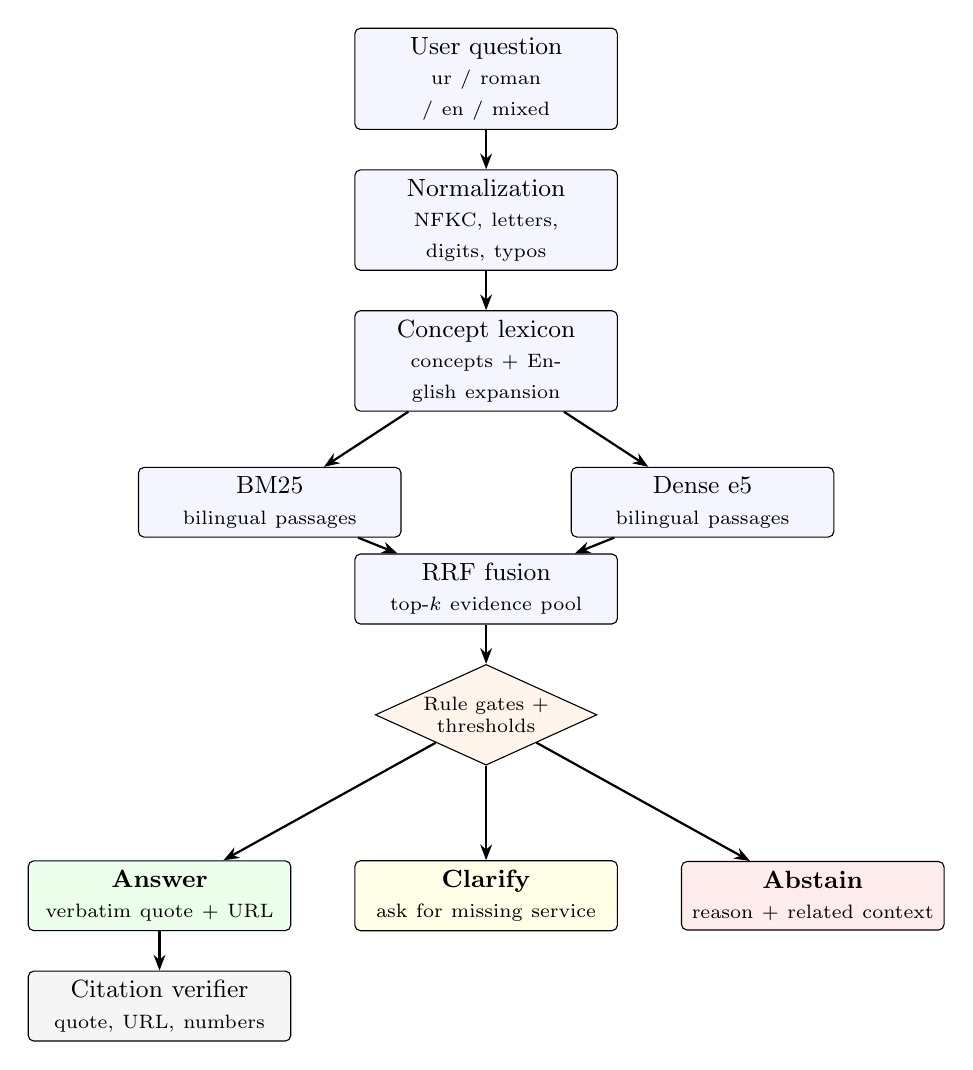
\begin{tikzpicture}[
  node distance=5mm and 6mm,
  box/.style={draw, rounded corners=2pt, align=center, font=\small, minimum height=8mm, text width=3.1cm, fill=blue!4},
  gate/.style={draw, diamond, aspect=2.2, align=center, font=\scriptsize, inner sep=1pt, fill=orange!8},
  outbox/.style={draw, rounded corners=2pt, align=center, font=\small, minimum height=8mm, text width=3.1cm},
  arr/.style={-{Stealth[length=2mm]}, thick}]
  \node[box] (q) {User question\\ \scriptsize ur / roman / en / mixed};
  \node[box, below=of q] (n) {Normalization\\ \scriptsize NFKC, letters, digits, typos};
  \node[box, below=of n] (c) {Concept lexicon\\ \scriptsize concepts + English expansion};
  \node[box, below left=7mm and -6mm of c] (bm) {BM25\\ \scriptsize bilingual passages};
  \node[box, below right=7mm and -6mm of c] (de) {Dense e5\\ \scriptsize bilingual passages};
  \node[box, below=18mm of c] (rrf) {RRF fusion\\ \scriptsize top-$k$ evidence pool};
  \node[gate, below=of rrf] (g) {Rule gates +\\ thresholds};
  \node[outbox, below=12mm of g, fill=yellow!10] (cl) {\textbf{Clarify}\\ \scriptsize ask for missing service};
  \node[outbox, left=8mm of cl, fill=green!8] (a) {\textbf{Answer}\\ \scriptsize verbatim quote + URL};
  \node[outbox, right=8mm of cl, fill=red!7] (ab) {\textbf{Abstain}\\ \scriptsize reason + related context};
  \node[box, below=of a, fill=gray!8] (v) {Citation verifier\\ \scriptsize quote, URL, numbers};
  \draw[arr] (q) -- (n); \draw[arr] (n) -- (c);
  \draw[arr] (c) -- (bm); \draw[arr] (c) -- (de);
  \draw[arr] (bm) -- (rrf); \draw[arr] (de) -- (rrf);
  \draw[arr] (rrf) -- (g);
  \draw[arr] (g) -- (a); \draw[arr] (g) -- (cl); \draw[arr] (g) -- (ab);
  \draw[arr] (a) -- (v);
\end{tikzpicture}
\caption{System architecture. Every answer is a verbatim quote of an official passage that has passed the citation verifier.}
\label{fig:flow}
\end{figure}

% =====================================================================================
\section{Dataset and Provenance}
We use the organisers' file \texttt{Multilingual\_E-Sahulat\_AI\_Hackathon\_Dataset.docx} as given: \RNRecords{} JSON
records, SHA-256 prefix \texttt{\RDatasetHash}.

\paragraph{Knowledge base.} The \RNPassages{} distinct official evidence excerpts (\texttt{F01}--\texttt{F30}) form the
corpus. Each passage keeps its \texttt{source\_url} on \texttt{dgip.gov.pk} (\RNDocs{} distinct pages), a document ID, an
authority tier, a text hash, and the dataset's Urdu evidence translation. The Urdu text is indexed for Urdu-script matching
and displayed in Urdu responses. The \emph{English official excerpt} is always the cited text. An optional notebook cell
downloads each live page and checks every passage fragment against it.

\paragraph{Query splits.} Table~\ref{tab:splits} lists the splits. The official \texttt{train\_dev} split contains no
unanswerable queries, so we wrote \RNDevAux{} negative development queries (out-of-domain, out-of-KB services, ambiguous,
personal, noise, injection, unsafe) and used them \emph{only} for threshold tuning.

\begin{table}[H]
\centering
\begin{tabularx}{\textwidth}{@{}l l c X@{}}
\toprule
Split & Source & $n$ & Use and contents \\
\midrule
Dev & official \texttt{train\_dev} & \RNDevOfficial & Lexicon design, retriever selection, threshold tuning. 30 intents $\times$ en / ur / roman\_ur. \\
Dev & team-written negatives & \RNDevAux & Threshold tuning only. \\
Test & official \texttt{test} & \RNTest & Reported once. 30 noisy Roman Urdu spelling variants plus 30 hard cases (ambiguous, personal, out-of-domain, injection, time-sensitive, conflicting, unsafe). \\
Brief & challenge Cases 1--12 & \RNBrief & Team-labelled gold, reported separately (Urdu, Roman, English, code-mixed, typo, paraphrase, Unicode variant, noise). \\
\bottomrule
\end{tabularx}
\caption{Query sets. Expected decisions: \textit{answer} (answerable, including partial), \textit{clarify} (ambiguous),
\textit{abstain} (all other unanswerable topics). For \textit{unsupported\_generalization}, either non-answer counts as correct.}
\label{tab:splits}
\end{table}

% =====================================================================================
\section{Methodology}

\subsection{Query Normalization}
All text, queries and passages alike, goes through the same meaning-preserving normalization:
(i) Unicode NFKC and removal of invisible characters; (ii) unification of Arabic-keyboard letters
(\textit{yeh}, \textit{kaf}, \textit{heh}, hamza-alef forms) to their Urdu code points; (iii) removal of diacritics and
\textit{tatweel}, conversion of Urdu and Arabic-Indic digits to ASCII, and mapping of Urdu punctuation;
(iv) lowercasing, collapsing letters repeated three or more times, and splitting digit-letter boundaries
(\textit{10saal} $\to$ \textit{10 saal}); (v) number words to digits (\textit{das}, \textit{ten} $\to$ 10).
The detected language style (Urdu script, Roman Urdu or English) matched the dataset labels for \RStyleAcc{} of official
queries.

\textbf{Spelling-variant repair.} A Latin token $w$ of at least five characters that is absent from the lexicon is replaced by
\begin{equation}
w^\ast = \arg\max_{v \in V_{\text{lex}}} \text{sim}(w, v) \quad \text{if} \quad \max_{v} \text{sim}(w, v) \geq 0.84,
\end{equation}
where $\text{sim}$ is the Ratcliff--Obershelp ratio, so \textit{documnts} becomes \textit{documents} and \textit{pasport}
becomes \textit{passport}. Known tokens are never rewritten.

\subsection{Cross-Script Concept Lexicon}
More than fifty concepts (e.g.\ \texttt{RENEW}, \texttt{MINOR}, \texttt{DUAL}, \texttt{FASTTRACK}, \texttt{REFUND}) list
their English, Roman Urdu and Urdu-script surface forms. A query $q$ yields a concept set $C(q)$ and an expansion
$E(q)=\bigcup_{c\in C(q)} \text{exp}(c)$ of English terms drawn from the corpus. Keyword retrievers then score
$q \oplus E(q)$, which lets an Urdu-script query match English evidence.

\subsection{Retrieval}
\textbf{Sparse retrieval (BM25).} Passages are scored with BM25Okapi ($k_1=1.5$, $b=0.75$):
\begin{equation}
\text{score}_{\text{BM25}}(q, d) = \sum_{t \in q} \text{IDF}(t) \cdot
\frac{f(t,d) \cdot (k_1+1)}{f(t,d) + k_1 \cdot \left(1 - b + b \cdot \frac{|d|}{\text{avgdl}}\right)}
\end{equation}
where $f(t,d)$ is the frequency of token $t$ in passage $d$, $|d|$ is the passage length and avgdl is the average passage
length. Passages with zero score are treated as not retrieved.

\textbf{Dense retrieval.} The query and each passage are embedded with \RDenseModel{} (with the
\texttt{query:}/\texttt{passage:} prefixes for e5) and ranked by cosine similarity:
\begin{equation}
\text{score}_{\text{dense}}(q, d) = \frac{\mathbf{e}_q \cdot \mathbf{e}_d}{\lVert \mathbf{e}_q \rVert \, \lVert \mathbf{e}_d \rVert}
\end{equation}

\textbf{Hybrid fusion.} Rankings are combined with Reciprocal Rank Fusion and an authority weight $w_{a(d)}$ (1.0 for
official sources, 0.8 for third-party ones):
\begin{equation}
\text{score}_{\text{RRF}}(d) = w_{a(d)} \sum_{r \in R} \frac{1}{60 + \text{rank}_r(d)}
\end{equation}

Nine configurations are compared (Table~\ref{tab:ret}): raw BM25, char n-gram TF-IDF, BM25 with normalization and the
lexicon (English or bilingual passages), dense retrieval (English, bilingual, bilingual + expansion) and two hybrids. The
\textbf{production retriever is chosen by development MRR@5}; the selection was \RFinalMethod.

\subsection{Decision Cascade, Abstention and Clarification}
Each query receives exactly one decision through the ordered gates in Table~\ref{tab:gates}.

\begin{table}[H]
\centering
\begin{tabularx}{\textwidth}{@{}c X l@{}}
\toprule
\# & Condition & Decision \\
\midrule
1 & No letters at all (noise) & abstain: no result \\
2 & Prompt injection (``ignore rules'', ``invent'', ``cite na karo'') & abstain: refuse \\
3 & Unsafe request (bypass verification, fake documents) & abstain: refuse \\
4 & Service outside the KB (visa, NADRA CNIC, driving licence, office hours) & abstain: out of scope \\
5 & Personal status, delivery prediction, guarantee, booking, ``still current today?'' & abstain + related context \\
6 & User claims conflicting sources & abstain + what the KB states \\
7 & Asks \emph{what / how much / how long} with no service named & clarify \\
8 & Fee amount with no other topic (no fee schedule in the KB) & clarify \\
9 & No domain concept and $s_{\text{dense}} < \tau_{\text{ood}}$ & abstain: out of scope \\
10 & $s_{\text{dense}} \geq \tau_d$ and $\text{cov} \geq \tau_c$ & \textbf{answer}; otherwise abstain \\
\bottomrule
\end{tabularx}
\caption{Decision cascade. Coverage $\text{cov}$ is the fraction of the query's content stems (including expansions) that
occur in the top passage.}
\label{tab:gates}
\end{table}

\textbf{Threshold tuning.} $(\tau_d, \tau_c, \tau_{\text{ood}})$ are grid-searched (\RTuneGrid{} combinations) on the
development split only, maximizing an objective that weights false answers more than missed answers:
\begin{equation}
J(\tau) = 0.4 \cdot \text{Recall}_{\text{answer}}(\tau) + 0.6 \cdot \text{Acc}_{\text{non-answer}}(\tau).
\end{equation}
The middle of the optimal plateau (\RTunePlateau{} tied points) is chosen for robustness, giving
$\tau_d=\RTauDense$, $\tau_c=\RTauCov$ and $\tau_{\text{ood}}=\RTauOOD$ (dev objective \RTuneObjective).

\subsection{Grounded Answer Generation and Citation Verification}
Answers are \textbf{extractive}: the top official passage is quoted verbatim with
\texttt{[ID] title <URL>}. In Urdu mode the dataset's Urdu evidence text is shown under the English quote, and in Roman
Urdu mode the framing messages are in Roman Urdu. A footer states that only the quoted text is verified. A verifier checks,
for every evidence item, that (a) the passage ID exists, (b) the URL equals the document registry entry, (c) the quoted span
is a substring of the passage and (d) every number in the span appears in the passage. Tamper tests (altered quote, wrong
URL, unknown ID) confirm that the verifier rejects fabricated citations.

\subsection{Conflict Handling}
Passages that state the same quantity share a \texttt{fact\_key}. If the top-$k$ pool contains different values for one key,
the response prefers the official (and, where dated, newer) source and discloses the disagreement. Because the official
KB contains no contradictions, this is demonstrated by injecting a clearly labelled \emph{synthetic} outdated passage into a
copy of the index. The synthetic passage is never used in any metric.

% =====================================================================================
\section{Evaluation Protocol}
For the answerable query set $Q_{\text{ans}}$ with gold passage set $G_q$ and ranking $\pi_q$:
\begin{align}
\text{Recall@5} &= \frac{1}{|Q_{\text{ans}}|}\sum_{q} \mathbb{1}\left[G_q \cap \pi_q[1..5] \neq \emptyset\right], \\
\text{MRR@5} &= \frac{1}{|Q_{\text{ans}}|}\sum_{q} \frac{1}{\text{rank}_q}, \qquad \frac{1}{\text{rank}_q} := 0 \text{ if } \text{rank}_q > 5.
\end{align}
The \textbf{citation support rate} is the share of answered queries with gold evidence whose citation both passes the
verifier and points to a gold passage. \textbf{Abstention} is reported as decision accuracy, answer precision and recall,
clarify accuracy, and the \textbf{false-answer rate} on unanswerable queries. \textbf{Cross-script consistency} measures
whether the English, Urdu and Roman Urdu versions of the same development question retrieve the same top passage, and whether
held-out noisy Roman Urdu test queries retrieve the same top passage as their English dev counterpart. \textbf{Latency} is
the end-to-end \texttt{respond()} time with the model loaded and all per-query caches cleared. Confidence intervals are
95\% percentile bootstraps over queries (2000 resamples).

% =====================================================================================
\section{Results}
All values in this section were generated by the notebook run that produced \texttt{results/} (dense backend:
\RDenseBackend; model: \RDenseModel).

\subsection{Retrieval}
\begin{table}[H]
\centering
\small
\restablefit{tab_retrieval_test}
\caption{Retrieval on the official test split ($n=\RNTestGold$ queries with a gold passage). The production retriever is
in bold; it was selected on development data before test was evaluated.}
\label{tab:ret}
\end{table}

\begin{table}[H]
\centering
\small
\restablefit{tab_retrieval_lang}
\caption{Recall@5 on the test split by query variant and language. ``spelling variant'' are the 30 noisy Roman Urdu
queries; ``hard case'' are the answerable hard cases.}
\label{tab:retlang}
\end{table}

\begin{figure}[H]
\centering
\resfig{retrieval_test.png}{0.9\textwidth}
\caption{Recall@5 and MRR@5 of all retrievers on the official test split.}
\label{fig:ret}
\end{figure}

\subsection{Cross-Script Consistency}
\begin{table}[H]
\centering
\small
\restablefit{tab_cross}
\caption{Cross-script consistency. Same top-1 and all hit@5 are over the 30 development intents asked in English, Urdu and
Roman Urdu; SV$\rightarrow$EN compares each noisy Roman Urdu test query with the English dev query of the same intent.}
\label{tab:cross}
\end{table}
End to end on dev, the same decision is reached for all three scripts in \REtoECrossDec{} of intents, and the same decision
\emph{and} the same citation in \REtoECrossCite.

\subsection{Answer Reliability, Abstention and Citations}
\begin{table}[H]
\centering
\small
\restablefit{tab_decisions}
\caption{Decisions, abstention and citation integrity.}
\label{tab:dec}
\end{table}

\begin{table}[H]
\centering
\small
\restablefit{tab_confusion}
\caption{Confusion matrix of expected versus produced decisions on the official test split.}
\label{tab:conf}
\end{table}

\begin{figure}[H]
\centering
\resfig{decisions_latency_test.png}{0.95\textwidth}
\caption{Left: test decision accuracy by topic. Right: distribution of end-to-end latency.}
\label{fig:dec}
\end{figure}

\subsection{Latency}
With the model loaded and per-query caches cleared, \texttt{respond()} takes p50 = \RLatPfifty{} ms, p95 =
\RLatPninetyfive{} ms and mean = \RLatMean{} ms per query on the test split.

% =====================================================================================
\section{Error Analysis}
Errors are tagged automatically as missed answers (threshold versus rule gate), false answers, clarify/abstain confusions,
or wrong passages (a \emph{confusable sibling} such as F13/F14/F15, or an unrelated passage). There were \RNErrors{} errors
across the test and brief sets (Table~\ref{tab:err}); Table~\ref{tab:fail} lists examples. Failure patterns to examine
include numeric qualifiers that appear in several passages (e.g.\ ``10-year validity'' in F12 versus ``below 10 years of
age'' in F06) and sibling passages that differ by one word (Normal / Urgent / Fast Track in F13--F15).
% Edit this paragraph after your final run to describe the failures you actually observed.


\begin{table}[H]
\centering
\small
\restable{tab_errors}
\caption{Error types on the test and brief sets.}
\label{tab:err}
\end{table}

\begin{table}[H]
\centering
\scriptsize
\restable{tab_failures}
\caption{Example failures (first eight).}
\label{tab:fail}
\end{table}

\subsection{Leakage Audit and Conservative Estimates}
\label{sec:leakage}
The official test queries were visible while the lexicon and rule gates were being designed. Numeric thresholds were tuned on
development data only, but the hand-written lexicon and cue phrases could still be fitted to test. We therefore audit:
\begin{itemize}
  \item \textbf{Lexicon forms} that occur in test queries but never in dev or corpus text: \RLeakForms{} forms. Removing them
        gives test Recall@5 = \RLeakRecallWithout{} and MRR@5 = \RLeakMRRWithout{} for the production retriever.
  \item \textbf{Rule-gate cue phrases} that fire on test queries but on no dev or brief query: \RLeakCues{} phrases. Removing
        them gives test decision accuracy = \textbf{\RCueAccWithout} and a false-answer rate on unanswerable queries of
        \textbf{\RCueFalseWithout}.
\end{itemize}
We regard these ablated figures as the \textbf{conservative estimate} on the official test, and the official test itself as a
regression suite. True generalization is measured on a blind set written by a team member who had not seen the code
(status: \RBlindStatus).

% =====================================================================================
\section{Validation Cases}
\begin{table}[H]
\centering
\small
\begin{tabularx}{\textwidth}{@{}l X X@{}}
\toprule
Case & Behaviour & Mechanism \\
\midrule
1--3 & Urdu / Roman / English renewal-documents question retrieves the same evidence & normalization, lexicon, bilingual index \\
4 & Code-mixed online-versus-office question & concept expansion, hybrid retrieval \\
5 & \textit{renew karwana hai} vs.\ \textit{renu karwana hy} & spelling repair; per-retriever RR reported \\
6 & Paraphrase (``replace my expired passport'') & dense retrieval \\
7 & Guaranteed processing time & guarantee / personal gate; abstain with context \\
8 & Cricket World Cup & no domain concept, $\tau_{\text{ood}}$ \\
9 & ``How much does it cost?'' & clarify: asks for passport type, pages, validity, service \\
10 & Conflicting sources & \texttt{fact\_key} conflict detection; synthetic demo \\
11 & Citation integrity & verifier on every answer; tamper tests \\
12 & Random strings & noise gate and evidence thresholds \\
\bottomrule
\end{tabularx}
\caption{The brief's validation cases and how the system handles them. The notebook (Step 8) prints each case's full
response. Decision accuracy on the brief set: \RBriefAcc.}
\label{tab:cases}
\end{table}

% =====================================================================================
\section{Observations and Insights}
\begin{itemize}
    \item Raw keyword retrieval fails on Urdu script because the official text is English; normalization plus the concept
          lexicon is the single largest improvement (Table~\ref{tab:ret}).
    \item Indexing the Urdu evidence text alongside the English passage helps Urdu-script queries without changing what is
          cited.
    \item Dense multilingual retrieval adds robustness to paraphrases, while lexicon expansion adds robustness to Roman Urdu
          spelling; the hybrid combines both.
    \item Extractive answering removes the main hallucination risk: every displayed claim is a verbatim official quote that
          passes the verifier.
    \item Most remaining errors are confusions between sibling passages that differ by a single number or qualifier.
\end{itemize}

\section{Limitations and Responsible Deployment}
\begin{itemize}
    \item \textbf{Small corpus:} with \RNPassages{} passages, retrieval resembles intent classification. Scaling to full
          DGI\&P pages requires chunking and re-evaluation.
    \item \textbf{Hand-built rules:} the lexicon and gates were written with the dataset in view (\S\ref{sec:leakage}).
    \item \textbf{No fee schedule:} fee amounts are not in the KB, so the system clarifies or abstains instead of quoting fees.
    \item \textbf{Freshness:} official procedures change, so passages must be re-verified against live pages before deployment.
    \item \textbf{Readability:} verbatim quotes are safe but less conversational; the Urdu translation is assistive, and the
          English official text remains authoritative.
\end{itemize}

\section{Practical Impact}
The assistant targets citizens who search in Roman Urdu or Urdu, including users with limited English, and gives them
official, citable answers instead of forum hearsay. Refusing to guess about fees, guarantees or individual cases reduces the
risk of misleading people about legal requirements. The same architecture (normalize, bridge, retrieve, verify, abstain)
transfers to CNIC, licensing or other e-Sahulat domains by swapping the corpus and extending the lexicon.

\section{Conclusion}
Multilingual E-Sahulat AI retrieves official passport evidence robustly across Urdu script, Roman Urdu, English and
code-mixed queries, answers only with verbatim, verified citations, and abstains or asks for clarification when the
evidence does not support an answer. The evaluation reports measured retrieval, consistency, reliability, citation and
latency figures together with an explicit leakage audit, so the claims can be checked against the notebook that produced
them.

\appendix
\section{Reproducibility}
\begin{itemize}
  \item Run the notebook top to bottom with the dataset file next to it; Step 10b writes \texttt{results/} for this report.
  \item Dataset SHA-256 prefix: \texttt{\RDatasetHash}. Random seed: 42.
  \item Dense model: \RDenseModel.
  \item Outputs (in \texttt{esahulat/outputs/}):
  \begin{itemize}
    \item \texttt{per\_query\_results.csv} and \texttt{error\_analysis.csv}
    \item \texttt{manual\_audit.csv} (human citation check)
    \item \texttt{results.json} and \texttt{results\_report.md}
  \end{itemize}
  \item Compile this report with \texttt{pdflatex report.tex} (run twice for the table of contents).
\end{itemize}

\end{document}
